
\section{Methodology}
\label{sec:methodology}

% ,,,,,,,,,,,,,,,,,,,,,,
\subsection{System overview and design rationale}
\label{sec:overview}
% ,,,,,,,,,,,,,,,,,,,,,,

This section describes the apparatus and the procedure. The
apparatus is a closed-loop measurement system: it reads two
physiological channels from a wearable sensor unit, reduces them
to a single continuous index of autonomic arousal calibrated
against the individual participant, and converts that index into
control messages that modulate an immersive virtual environment.
The procedure is the sequence each session follows, from sensor
placement through a fixed calibration window to the recorded run.

Two raw channels enter the system and three derived quantities
leave it. Heart rate and heart-rate variability are obtained from
the electrocardiogram; the phasic component of electrodermal
activity is obtained from the skin conductance channel. Each is
expressed as a deviation from the same participant's resting
values, standardised against the dispersion observed during that
participant's own calibration window, and combined into a single
weighted composite. Two thresholds, fixed at the close of
calibration and held constant thereafter, partition the composite
into three states, and the state determines which of four messages
the virtual environment receives.

Physiological measurement, per-participant calibration, index
computation, and immersive presentation are four separable
problems, and a system fusing them into a single codebase
inherits the constraints of all four at once. We separated the
layers instead. The measurement system runs as a server and each
virtual environment connects to it as a client. Two channels
carry everything passing between them: short command strings
travel outward from server to environment, and structured
telemetry travels back. Neither channel encodes anything
scenario-specific. The server learns which environment is
connected only from the label in its telemetry, and admitting a
new scenario requires no modification to it.

What follows from this is that a single measurement apparatus
serves several scenarios on identical instrumentation, under
identical calibration procedure and identical index arithmetic.
Comparisons across scenarios therefore rest on a common
measurement basis rather than on separately implemented
approximations of one.

The same separation extends beneath the contract. The sensor unit
is reached through a data-source adapter that publishes a fixed
three-channel stream, so a different acquisition device needs a
new adapter and nothing else. Extraction of heart rate,
variability and phasic conductance sits behind an interface with
two independent implementations already in place
(Section~\ref{sec:backends}). The columns of the session record
are learned from the environment at run time rather than declared
in advance. What the framework fixes is deliberately small: two
network channels, four commands, one telemetry envelope, one
calibration procedure and one index. Everything else is free to
vary, and is expected to.

We claim no novelty for the individual processing steps.
Detection, variability estimation and the separation of the
conductance signal rely on published libraries and standards, and
the composite combines their outputs under coefficients fixed in
advance rather than fitted to recorded data.

The contribution reported here is accordingly the framework
itself: the apparatus, its calibration, its decision rule and its
record, specified closely enough to be reproduced. Data collection
under the protocol is in progress, and outcomes for any particular
exposure scenario lie outside the scope of this account.

The account below follows the signal. The modular structure is
set out first, followed by the apparatus and software environment,
the acquisition of each physiological quantity together with the
two implementations that derive it, calibration, the composite
index, and classification with its control law. The interface to
the environment, the session procedure and the monitoring
arrangements come next, then what is written to disk, how the
system is validated and reproduced, and finally the arrangements
for ethics and data protection.

% ,,,,,,,,,,,,,,,,,,,,,,
\subsection{Architecture and modularity}
\label{sec:modularity}
% ,,,,,,,,,,,,,,,,,,,,,,

Every substitutable component in the system is substitutable at
exactly one location. This is not an aesthetic preference. It is
the property permitting a single laboratory to support several
scenarios, to replay archived recordings through the live
pipeline, and to hold two independent signal-processing libraries
against one another on identical input. Four axes of substitution
are provided.

\textbf{Data source.} One configuration constant selects between
a live sensor unit and an archived recording replayed at its
original rate. Both publish the same three-channel stream, so no
module downstream of the selection is able to distinguish them.
Development, regression testing and offline analysis therefore
exercise the same processing a live session uses.

\textbf{Extraction backend.} Two implementations of the cardiac
and electrodermal derivations coexist behind a common interface.
The default calls NeuroKit2~\citep{makowski2021}; the alternative
follows the routines published with the sensor vendor's own
analysis package~\citep{plux2020}. Selection is made in
configuration, and the arithmetic downstream of extraction is
shared in full. Section~\ref{sec:backends} treats this at length.

\textbf{Virtual environment.} The interface presented to the
environment is fixed and scenario-neutral. Any environment
consuming four command strings and emitting telemetry in the
shared envelope is a valid client. Both the scenario label and
the telemetry field names are learned at run time from the first
packet received, so neither the control loop nor the record
carries scenario-specific code. The only scenario names in the
system are optional display hints telling the console which field
to chart for the three current scenarios, together with a channel
kept from the first scenario that forwards the balloon height to
the console.

\textbf{Recording schema.} Columns in the session record are
established from the first telemetry packet rather than declared
in advance. A scenario reporting two fields absent from every
other scenario contributes two columns, and no modification to
the recording code is required. Should no environment connect at
all, the header commits with the physiological columns alone and
the recording proceeds.

Each of these is a single editable location. Taken together they
mean that a study changing scenario, changing extraction library,
or substituting archived input for live capture is reconfigured
in minutes rather than reimplemented.

\begin{figure}[H]
    \centering
    \IfFileExists{diagrams/01_system_topology.png}{%
        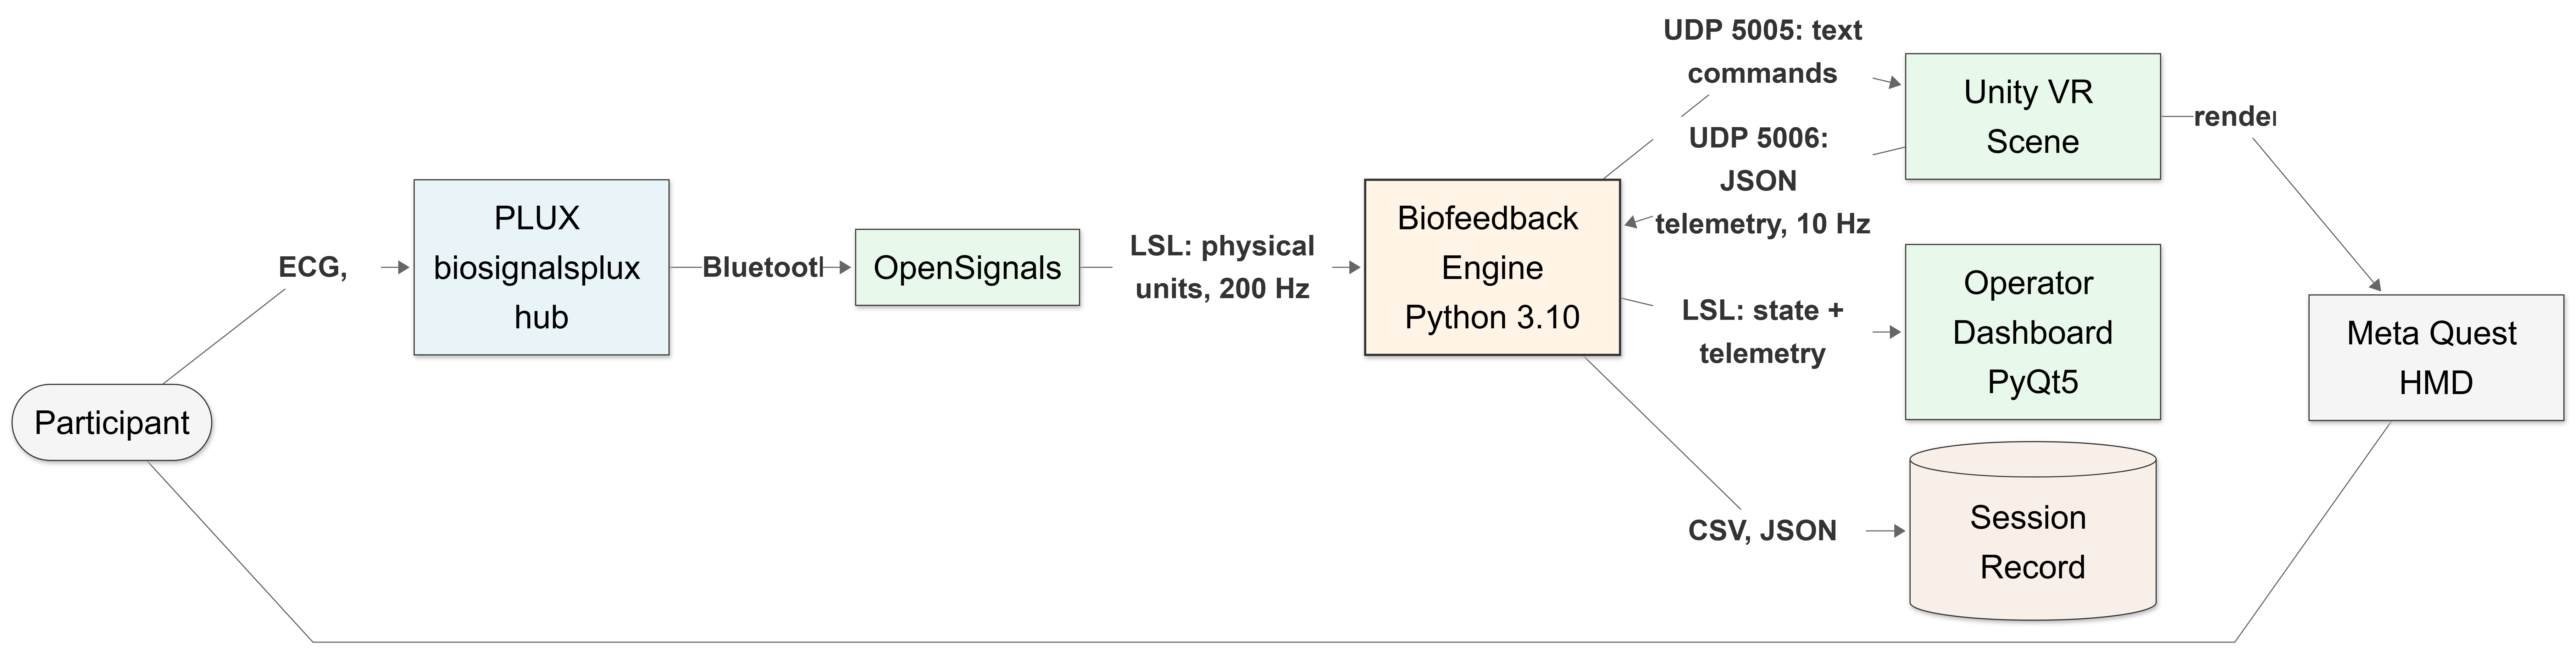
\includegraphics[width=\linewidth]{diagrams/01_system_topology.png}%
    }{%
        \fbox{\parbox{0.9\linewidth}{\centering
            \vspace{1.5cm}
            \textbf{[Diagram 1 placeholder, system topology]}\\[6pt]
            \small Render the corresponding mermaid source and place
            the exported image in \texttt{diagrams/}.
            \vspace{1.5cm}
        }}%
    }
    \caption{System topology. Physiological signals enter through
    the wearable unit, reach the measurement server over the Lab
    Streaming Layer, and modulate the virtual environment through
    a command channel. Telemetry returns on a second channel.
    Recording proceeds in parallel with the control loop.}
    \label{fig:topology}
\end{figure}

\begin{figure}[H]
    \centering
    \IfFileExists{diagrams/02_multi_scenario_contract.png}{%
        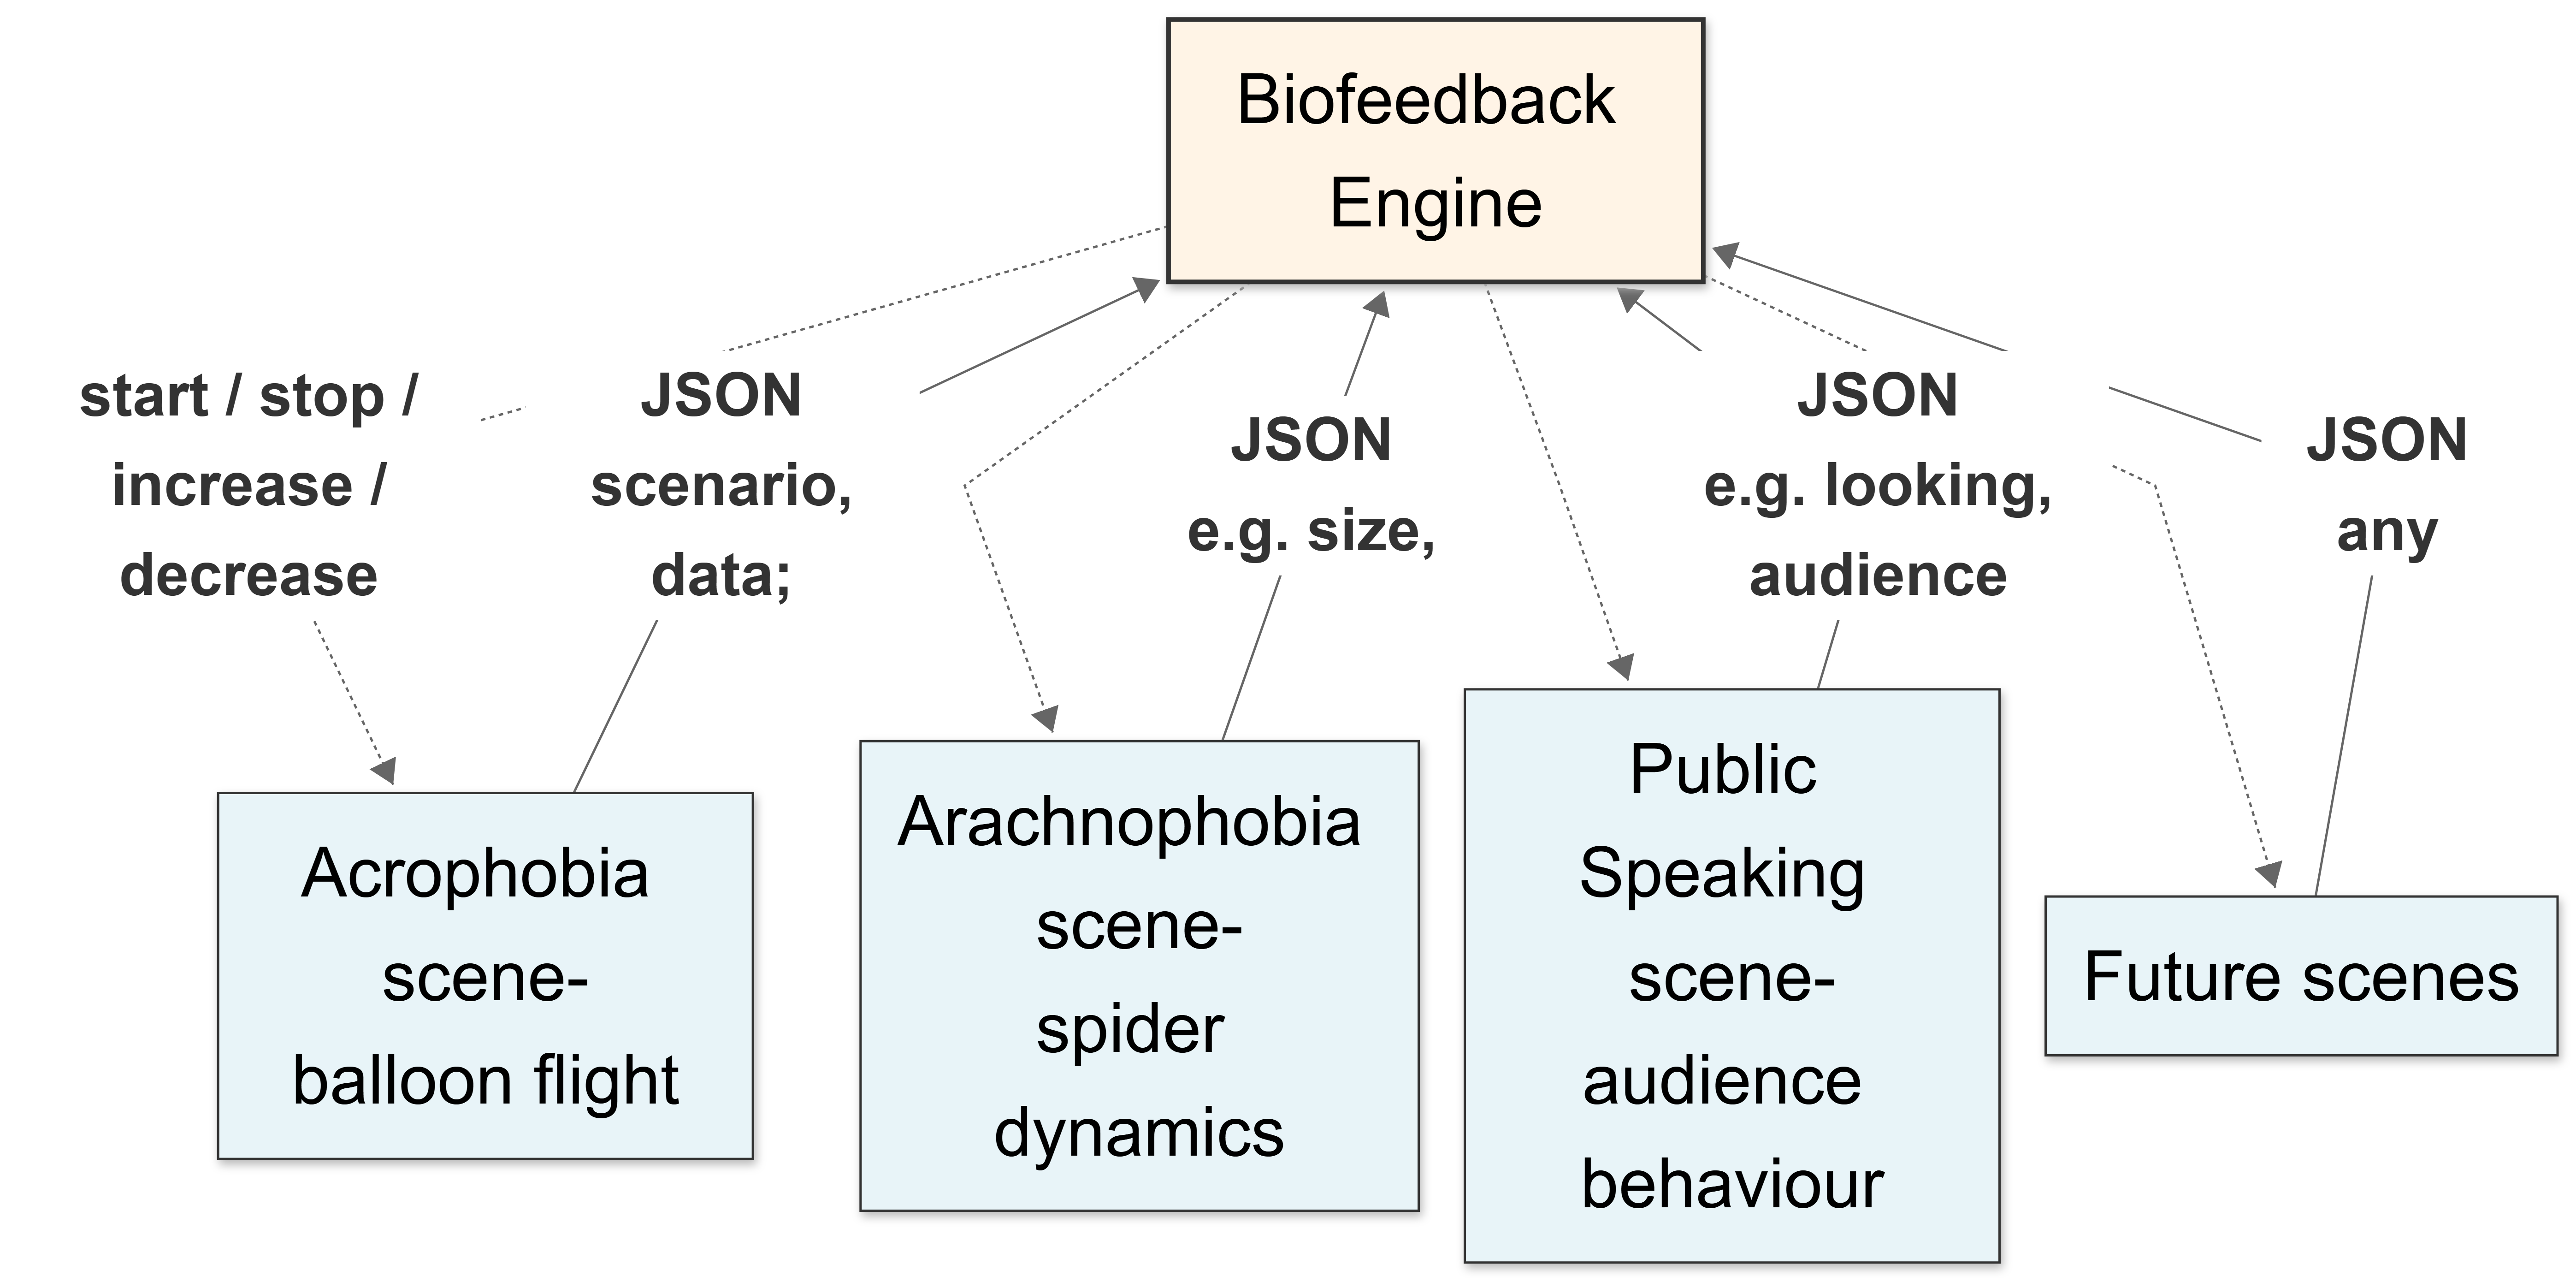
\includegraphics[width=\linewidth]{diagrams/02_multi_scenario_contract.png}%
    }{%
        \fbox{\parbox{0.9\linewidth}{\centering
            \vspace{1.5cm}
            \textbf{[Diagram 2 placeholder, scenario interface]}\\[6pt]
            \small Render the corresponding mermaid source and place
            the exported image in \texttt{diagrams/}.
            \vspace{1.5cm}
        }}%
    }
    \caption{The scenario-neutral interface. One server drives any
    number of environments through four command strings. Telemetry
    returns in a single envelope whose inner fields differ by
    scenario and are recorded without being declared in advance.}
    \label{fig:contract}
\end{figure}

% ,,,,,,,,,,,,,,,,,,,,,,
\subsection{Apparatus}
\label{sec:apparatus}
% ,,,,,,,,,,,,,,,,,,,,,,

\subsubsection{Sensing hardware and electrode placement}
\label{sec:sensing}

Each participant wears a wireless biosignal unit (biosignalsplux,
PLUX Wireless Biosignals, Lisbon) secured on an elastic chest
band. Two sensor assemblies connect to it.

Cardiac activity is recorded through a three-lead
electrocardiography cable in the standard Lead~I configuration:
positive electrode at the left mid-clavicular line, negative
electrode at the corresponding position on the right, reference
electrode on the lower left rib margin. Disposable pre-gelled
Ag/AgCl electrodes are used. The skin is cleaned with alcohol and
allowed to dry before application.

Electrodermal activity is recorded through a two-electrode
assembly on the intermediate phalanges of the index and middle
fingers of the non-dominant hand. The non-dominant hand is chosen
so the dominant hand remains free for whatever interaction the
scenario requires. The digital site is chosen because palmar and
digital eccrine glands receive sympathetic innervation without a
parasympathetic counterpart, which makes conductance measured
there an unusually direct index of sympathetic activity
\citep{boucsein2012, dawson2016}.

Both channels are digitised at 1000~Hz with 16-bit resolution
against a 3~V reference. The rate is dictated by the cardiac
channel. Variability is computed from the intervals between
successive R~peaks, so any error in placing a peak enters every
successive difference, and the standards document accordingly
recommends sampling the electrocardiogram at 250 to 500~Hz or
higher whenever beat-to-beat intervals are to be
analysed~\citep{taskforce1996}; at 1000~Hz each peak is placed to
within a millisecond. The same rate far exceeds what electrodermal
activity demands, since a skin conductance response evolves over
seconds, and sampling both channels at one common rate removes any
need to resample before they are combined. The system reads the
rate from the incoming stream rather than assuming it, so a unit
configured to a different rate is processed by identical code.

The unit transmits over Bluetooth to a workstation,
where the vendor capture application publishes samples on the Lab
Streaming Layer~\citep{kothe2019}\footnote{Open source, at
\url{https://github.com/sccn/labstreaminglayer}.}, from which any
local process may subscribe. Our system is one such subscriber.

The capture application publishes values already
converted into physical units, microsiemens for conductance and
millivolts for cardiac potential, rather than the raw converter
integers its published examples imply. A configuration
constant now selects between the two conventions, so archived
recordings carrying raw integers and live sessions carrying
physical units are handled by identical code.

\subsubsection{Immersive display}
\label{sec:display}

The virtual environment is presented through a Meta Quest
head-mounted display tethered to the workstation. Rendering is
performed on the workstation and the tether carries rendered
frames. Communication between the measurement system and the
rendering process uses local network sockets and is independent
of the tether, so the two subsystems fail independently. Nothing
in the measurement or control arrangement depends on the
particular display model.

\subsubsection{Software environment and versions}
\label{sec:versions}

The exact version of every dependency is recorded. This carries
more weight here than in ordinary application code, because
signal-processing libraries revise filter defaults and
peak-detection heuristics between minor releases, and a change of
that kind would shift derived values between a pilot run and a
final one without any edit to our own source.
Table~\ref{tab:versions} records the versions used throughout.

\begin{table}[H]
    \centering
    \renewcommand{\arraystretch}{1.4}
    \setlength{\tabcolsep}{10pt}
    \small
    \begin{tabular}{@{}p{3.0cm}p{2.0cm}p{8.0cm}@{}}
        \toprule
        \textbf{Component} &
        \textbf{Version} &
        \textbf{Function} \\
        \midrule
        Python & 3.10.11 & host language and runtime for all modules below \\
        \addlinespace[4pt]
        pylsl & 1.16.2 & Lab Streaming Layer client; publishes and subscribes to the internal three-channel stream \\
        \addlinespace[4pt]
        numpy & 1.22.2 & numerical core; signal arrays, calibration statistics, composite arithmetic \\
        \addlinespace[4pt]
        scipy & 1.8.1 & high-pass, powerline and low-pass filtering underlying both extraction backends \\
        \addlinespace[4pt]
        pandas & 2.0.3 & offline review of session records \\
        \addlinespace[4pt]
        neurokit2 & 0.2.13 & default extraction backend for heart rate, RMSSD and phasic conductance \\
        \addlinespace[4pt]
        biosignalsnotebooks & 0.6.14 & alternative extraction backend following the manufacturer's routines \\
        \addlinespace[4pt]
        PyQt5 & 5.15.11 & operator console framework and pre-session dialogue \\
        \addlinespace[4pt]
        pyqtgraph & 0.14.0 & live plotting at the pipeline rate \\
        \addlinespace[4pt]
        matplotlib & 3.8.4 & offline review figures \\
        \addlinespace[4pt]
        openpyxl & 3.1.5 & spreadsheet mirror of the session record with frozen header \\
        \addlinespace[4pt]
        Unity & 6000.3.0f1 & renders the virtual environment in a separate process \\
        \addlinespace[4pt]
        OpenSignals & vendor build & capture application supplied with the sensor unit \\
        \bottomrule
    \end{tabular}
    \caption{Software components, their versions, and the function
    each serves. Versions are those of the Python 3.10 virtual
    environment from which the system runs. The rendering process
    and the capture application run separately on the same
    workstation.}
    \label{tab:versions}
\end{table}

The manufacturer's analysis package is imported directly by the
alternative backend. Should it fail to load, the system reports
the failure once and falls back to the default backend rather than
stopping. Display firmware is absent from the table, as the
measurement system never addresses the display directly.

\subsubsection{Instrument selection}
\label{sec:tools}

Each component has established alternatives, and in most cases
selection rested on prior laboratory experience or on a specific
technical property.
Table~\ref{tab:tools} records what was chosen, what else was
available, and why.

\begin{table}[H]
    \centering
    \renewcommand{\arraystretch}{1.45}
    \setlength{\tabcolsep}{7pt}
    \small
    \begin{tabular}{@{}p{2.9cm}p{2.9cm}p{3.9cm}p{4.3cm}@{}}
        \toprule
        \textbf{Role} & \textbf{Selected} & \textbf{Alternatives}
            & \textbf{Basis for selection} \\
        \midrule
        Sensor unit &
            biosignalsplux &
            Shimmer3, BITalino, Empatica E4 &
            available in the laboratory; synchronous 1000~Hz capture
            on both channels at 16-bit resolution \\
        \addlinespace[7pt]
        Signal transport &
            Lab Streaming Layer \citep{kothe2019} &
            MQTT, ZeroMQ, ROS topics &
            sample-accurate timestamps across independent
            producers; established in neurophysiological practice \\
        \addlinespace[7pt]
        Extraction, default &
            NeuroKit2 \citep{makowski2021} &
            BioSPPy, HeartPy, MNE-Python &
            widest coverage; phasic separation of conductance
            included; artifact correction built in \\
        \addlinespace[7pt]
        Extraction, alternative &
            vendor routines \citep{plux2020} &
            as above &
            published by the sensor manufacturer; provides an
            independent implementation for cross-checking \\
        \addlinespace[7pt]
        R-peak detection &
            NeuroKit2 detector with correction
                \citep{lipponen2019} &
            Pan and Tompkins \citep{pantompkins1985}, Hamilton,
            Engzee &
            interpolates omitted beats before they can contaminate
            the variability estimate \\
        \addlinespace[7pt]
        Conductance decomposition &
            0.05~Hz high-pass filter &
            cvxEDA \citep{greco2016}, Ledalab, low-pass subtraction &
            library default; closed form, needs no optimisation
            solver \\
        \addlinespace[7pt]
        Rendering &
            Unity 6 \citep{unity2024} &
            Unreal Engine, Godot, WebXR &
            existing asset base and prior familiarity \\
        \addlinespace[7pt]
        Control transport &
            UDP sockets &
            WebSocket, gRPC, TCP &
            minimal overhead for single-shot messages; tolerance to
            loss already supplied by rate limiting \\
        \addlinespace[7pt]
        Operator console &
            PyQt5 with pyqtgraph &
            Tkinter, Dear PyGui, browser-based &
            native redraw performance at the pipeline rate \\
        \bottomrule
    \end{tabular}
    \caption{Instrument selection across the system. Extraction
    appears twice because both implementations remain active and
    are selected in configuration.}
    \label{tab:tools}
\end{table}

Two public benchmarks anchor this design space without being used
directly. WESAD~\citep{schmidt2018} supplies a multimodal
recording of chest and wrist physiology under laboratory stressors
and is the usual comparator when classifier variants are
validated. \citet{alberdi2016} survey multimodal stress
recognition more broadly, establishing which signal combinations
have historically proved informative and under what conditions.

% ,,,,,,,,,,,,,,,,,,,,,,
\subsection{Physiological measures}
\label{sec:measures}
% ,,,,,,,,,,,,,,,,,,,,,,

Two raw channels yield three derived quantities. Because the
remainder of this section refers to them constantly, each is
defined here along with its physiological basis.

\textbf{The electrocardiogram} records the electrical activity of
the heart at the skin surface. Each cardiac cycle produces the
characteristic P, QRS and T deflections. Only the QRS complex
concerns us: its R~peak is a sharp, reproducible landmark, and
every cardiac quantity we derive is computed from the intervals
between successive R~peaks rather than from the waveform itself.

\textbf{Heart rate} is the rate of beats implied by the intervals
between successive R~peaks, expressed in beats per minute. It
reflects the momentary balance between sympathetic acceleration
and parasympathetic deceleration at the sinoatrial node. Heart
rate is not specific to affective arousal: postural change and
physical effort move it as readily as psychological state does,
which is why it receives the smallest weight in the composite
defined in Section~\ref{sec:composite}.

\textbf{Heart-rate variability} is the beat-to-beat fluctuation
in those same intervals. We report RMSSD, the root mean square of
successive differences, which is the most widely used
time-domain measure over short recordings and is dominated by
vagal influence. Sympathetic activation withdraws vagal tone and
RMSSD falls accordingly, an association with a substantial
validation literature \citep{taskforce1996, thayer2012, kim2018}.

\textbf{Electrodermal activity} is the electrical conductance of
the skin, which varies with eccrine sweat gland activity. It
comprises two components on quite different timescales. The tonic
level drifts over minutes and reflects hydration, ambient
temperature and general arousal. Superimposed on it are discrete
responses lasting seconds, each corresponding to a sympathetic
event. Only the phasic component is informative for
moment-to-moment measurement, and the decomposition separating
the two is described in Section~\ref{sec:eda}.

% ,,,,,,,,,,,,,,,,,,,,,,
\subsection{Signal acquisition and conditioning}
\label{sec:acquisition}
% ,,,,,,,,,,,,,,,,,,,,,,

Samples arrive on the stream and pass three checks before any
subsequent arithmetic is applied to them.

\textbf{Validity bounds.} Values falling outside physiologically
plausible limits are rejected as sensor artifact rather than
accepted as measurement. Conductance is bounded to
$[0, 80]~\mu$S, heart rate to $[30, 220]$ beats per minute, and
RMSSD to $[0, 500]$~ms. A conductance value outside its bound
rejects the whole sample, whereas a heart rate or RMSSD outside its
bound is rejected for that quantity alone; in either case the most
recent valid value is held in place of the rejected one, so that no
downstream computation encounters an implausible input. A heart
rate or RMSSD that does not yet exist, as in the first minute after
the unit connects, is passed on as undefined rather than rejected.
These bounds are deliberately wide: they are set to catch
electrode detachment, converter faults and frank corruption, not
to exclude genuine physiological extremes.

\textbf{Continuity check.} Should the variance of any channel
collapse below a small threshold for longer than fifteen seconds,
the system infers electrode detachment or cable disconnection and
logs a warning. It does not terminate the session. A
detached electrode produces exactly this signature, and the
warning is intended to prompt inspection rather than to abort a
run that may still be recoverable.

\textbf{Rate cascade.} Several rates operate in the system and are
deliberately decoupled. The unit samples at 1000~Hz, and the
cardiac quantities are extracted at that native rate. Internal
processing advances at 10~Hz, which is ample given that both
cardiac quantities carry their own trailing-window estimators
beneath, and the phasic conductance estimate is drawn from a
window held at the same rate. Outbound commands are limited
to at most one per second, because more frequent modulation of the
environment is perceived as mechanical rather than as responsive.
Each rate is set in one location, and the acquisition rate is read
from the stream itself.

\subsubsection{Data source: live capture and archived replay}
\label{sec:data-source}

Two data sources feed the same three-channel stream, and one
configuration constant selects between them. No module downstream
of that selection can distinguish one from the other.

\textbf{Live capture} is the configuration used with a
participant present. Before the session opens, the launcher
confirms that the stream published by the capture application can
be found, and refuses to start otherwise. The system then
subscribes to that stream, reads its sampling rate from the stream
description, and identifies the cardiac and conductance channels by
label, falling back to their signal content when labels are absent.
Heart rate and RMSSD are computed from a rolling electrocardiogram
buffer within the same process. With every incoming sample the
latest conductance, heart rate and RMSSD are published together on
the internal stream, from which the acquisition stage takes the
most recent values at each 10~Hz step and applies the checks above;
phasic conductance is separated later in the pipeline. A watchdog
on the wireless link warns after two seconds of silence and ends
the session after fifty.

\textbf{Archived replay} substitutes a previously recorded
capture file for the live unit. The replay source parses the
header block to recover sampling rate and channel ordering, which
is not constant across files, derives heart rate and RMSSD for
the whole file in advance on the same windows and cadence used in
live capture, and then emits samples at the original rate into the
same stream the live source publishes on. Calibration, fusion,
classification and recording proceed exactly as they would with a
participant present.

Replay is not merely a development convenience. It is the
mechanism making the extraction chain falsifiable: because both
backends can be driven from byte-identical input, any divergence
between their outputs is attributable to the extraction
implementation and to nothing else. The agreement figures
reported in Section~\ref{sec:results-backends} are obtained this way, and
the same route is open to anyone wishing to validate a third
implementation, or to evaluate their own extraction code against
a recorded file without access to the hardware.

One defect in reproducibility is worth recording. On short files
the replay source formerly began emitting before the consuming
module had subscribed, so a variable number of leading samples
were lost and the calibration window differed between runs of
identical input. The replay source now waits up to ten seconds
for the consumer to subscribe before emitting, and identical input
now yields identical output.

\subsubsection{Extraction backends}
\label{sec:backends}

Two independent implementations of the extraction arithmetic are
maintained in parallel. Together with the archived replay described
above, they let the system be exercised, checked and reproduced
without depending on any single component being correct or even
present.

\textbf{The first backend follows the procedure prescribed by the
sensor manufacturer.} The routines published alongside the
capture application~\citep{plux2020} define how the manufacturer
intends its own recordings to be processed: detection by the Pan
and Tompkins method~\citep{pantompkins1985}, variability from
the interval series after the manufacturer's ectopy rule, and
conductance passed on as its raw level or, as a setting, with a
low-pass estimate of the tonic level at the conventional 0.05~Hz
boundary subtracted. Implementing this path means the
derived quantities can be reconciled against the manufacturer's
own documentation and against any analysis another laboratory
performs using the same published routines.

\textbf{The second backend is an independent general-purpose
package.} NeuroKit2~\citep{makowski2021} implements the same
operations with different algorithmic choices: its own detector
with the artifact correction of \citet{lipponen2019} in place of
uncorrected Pan and Tompkins, and a high-pass separation of the
phasic component in place of the raw level. It was
developed independently of the sensor hardware and shares no code
with the manufacturer's routines.

The reason for carrying both is that a derived quantity produced
by exactly one implementation cannot be distinguished from an
artifact of that implementation. Two independent paths over the
same input make the distinction available: agreement indicates
the quantity is a property of the signal, and disagreement
localises the discrepancy to a specific algorithmic choice rather
than leaving it unattributed. This matters more here than it
would for a single-scenario study, because the same measurement
apparatus is intended to serve several scenarios and any
systematic bias would propagate to all of them.

Selection is made in configuration, separately for the cardiac
quantities and for conductance, with a further setting choosing
how the manufacturer path treats conductance. The switch governs
only how the three input quantities are derived from the raw
channels; calibration, standardisation, weighting, smoothing,
threshold derivation and the control law are shared in full and
are unaffected by it. A session run under either backend is
therefore directly comparable to a session run under the other in
every respect except extraction.

The general-purpose package is the default, on two grounds. It
separates the phasic component of conductance by default, for the
reasons Section~\ref{sec:eda} sets out. It also incorporates
artifact correction, which handles omitted beats more robustly
than uncorrected detection.

Two further packages occupy this space, BioSPPy and HeartPy, each
well maintained and substitutable behind the same interface with
modest adapter code. Neither was adopted, as both overlap
functionally with what is already carried and the cross-checking
argument is satisfied by two independent implementations rather
than improved by a third.

\subsubsection{Cardiac measures}
\label{sec:hr-hrv}

In the default backend the raw electrocardiogram first passes a
fifth-order Butterworth high-pass filter at 0.5~Hz, which removes
baseline wander, and a powerline filter at 50~Hz, which removes
mains interference. The alternative backend passes the raw signal
directly to the Pan and Tompkins detector~\citep{pantompkins1985},
whose own band-pass stage serves the same purpose.

Detection follows. Both backends produce a series of R-peak
indices. The default combines the NeuroKit2 detector with the
correction procedure of \citet{lipponen2019}, which interpolates
omitted beats before they reach the variability computation. The
alternative applies the Pan and Tompkins detector without
interpolation.

Heart rate over a window is the mean of the instantaneous rates
given by successive peaks:

\begin{equation}
\mathrm{HR} \;=\; \frac{1}{N} \sum_{i=1}^{N}
\frac{60 \cdot f_{s}}{\Delta R_{i}}
\qquad \text{[beats per minute]}
\end{equation}

where $\Delta R_{i} = R_{i+1} - R_{i}$ is the difference in
sample index between successive R~peaks and $f_{s}$ is the
sampling rate. The alternative backend instead divides 60 by the
mean interval. Heart rate is recomputed every 0.5~s over a
trailing 30~s window and held between recomputations.

Variability is quantified as the root mean square of successive
differences between adjacent intervals:

\begin{equation}
\mathrm{RMSSD} \;=\; \sqrt{\frac{1}{N-1}
\sum_{i=1}^{N-1} \bigl( \mathrm{RR}_{i+1} - \mathrm{RR}_{i} \bigr)^{2}}
\qquad \text{[ms]}
\end{equation}

with intervals expressed as
$\mathrm{RR}_{i} = 1000 \cdot \Delta R_{i} / f_{s}$. RMSSD is
recomputed on the same 0.5~s cadence as heart rate but over a
trailing window of 60~s. In the default backend the window must
contain at least ten peaks, intervals outside 300 to 1500~ms are
discarded, and an estimate outside 5 to 300~ms is treated as a
detector failure, the previous value being held in its place.

That 60~s window is a considered choice between two positions in
the literature. The standards document~\citep{taskforce1996}
recommends 300~s for short-term variability. Work on shorter
recordings shows that RMSSD needs far less: comparing recordings
of 10, 30 and 120~s with recordings of four to five minutes in
3,387 adults, \citet{munoz2015} found agreement already
substantial for a single 10~s recording ($r \approx 0.85$) and
near perfect at 120~s ($r = 0.99$), and the review of
\citet{shaffer2017} reports acceptable agreement between
one-minute and five-minute RMSSD. A 60~s window lies within that
range while still following changes over a run of a few minutes,
which a 300~s window could not.

A relative-change criterion, attributable to Malik and colleagues
within the same standards document~\citep{taskforce1996},
governs which intervals contribute. Following correction, each
interval is compared against its predecessor and any pair whose
relative change exceeds 20\% is excluded:

\begin{equation}
\text{retain } \Delta \mathrm{RR}_{i}
\;\text{ if }\; \frac{\lvert \mathrm{RR}_{i+1} -
\mathrm{RR}_{i} \rvert}{\mathrm{RR}_{i}} \le 0.20
\end{equation}

The reasoning is direct. Ectopic beats surviving correction are
by construction outliers in the successive-difference series, and
because RMSSD squares those differences a single survivor inflates
the estimate substantially. A relative criterion is preferable to
an absolute one because tolerable beat-to-beat change scales with
rate. The alternative backend applies instead the ectopy rule of
\citet{lippman1994}, a differently formulated expression of the
same principle, and none of the bands above.

\subsubsection{Electrodermal measures}
\label{sec:eda}

Separating the two components of the conductance signal
determines what the composite is permitted to measure, so the
decomposition is described in some detail.

The \textbf{tonic} component, or skin conductance level, drifts
over minutes and reflects electrode hydration, ambient
temperature, resting arousal and elapsed time since application.
It carries almost no information at the timescale of interest.
Admitting raw conductance into the composite means admitting a
minutes-scale drift that overwhelms everything else: on our
early recordings tonic drift accounted for approximately 99\% of
the variance of the raw channel and dominated the composite
entirely when raw conductance entered at the weight given in
Section~\ref{sec:composite}.

The \textbf{phasic} component consists of discrete skin
conductance responses superimposed on the tonic level. Each
corresponds to a single sympathetic event, rises over roughly one
to three seconds, returns towards baseline over three to ten
seconds, and rarely exceeds a few tenths of a microsiemens. This
is the component carrying the information the composite requires
\citep{boucsein2012, dawson2016, fowles1980}.

The default backend separates the two with the filter NeuroKit2
applies by default. Conductance first passes a fourth-order
Butterworth low-pass filter at 3~Hz. A second-order Butterworth
high-pass filter at 0.05~Hz then removes the tonic level, leaving
the phasic component, and both filters run forwards and backwards
so that neither shifts the signal in time. The convex
decomposition of \citet{greco2016}, which the same library also
provides, is not used.

Every 0.5~s the filters are applied to the most recent 60~s of
conductance, held at the 10~Hz pipeline rate, and the final sample
of the phasic output becomes the current value entering the
composite. A first value is produced once five seconds of
conductance have accumulated.

\paragraph{Artifact handling on the conductance channel.} Four
distinct patterns appear in practice, each addressed at a
different stage.

\begin{itemize}
    \item \textbf{Values outside bounds.} A raw sample below zero
    or above 80~$\mu$S indicates electrode detachment or a
    converter fault rather than measurement. The sample is
    rejected and the last valid value is held in its place.
    Profuse sweating reaches approximately 50~$\mu$S, so the
    upper bound leaves genuine physiology considerable margin.
    \item \textbf{Converter saturation.} A saturated 16-bit
    value converts to exactly 25.0~$\mu$S under the calibration
    constants in use. That value lies within the bounds and is
    not rejected; a calibration resting at it is reported to the
    operator as degraded, as described in
    Section~\ref{sec:validity}.
    \item \textbf{Electrode detachment.} Variance collapse
    sustained beyond fifteen seconds is logged as a possible
    detachment, and the session continues pending operator
    inspection.
    \item \textbf{Values at the edge of the filter.} The phasic
    output occasionally exceeds 1~$\mu$S in magnitude at its
    final sample, where the forward and backward filter has no
    later samples to constrain it. Genuine responses rarely reach
    that magnitude, so any phasic value above 1~$\mu$S is
    rejected rather than repaired, since a repair rule risks
    misfiring on genuine high-magnitude data. The rejection is logged and the
    previous valid value is held.
\end{itemize}

The alternative backend separates nothing by default: it passes
the raw conductance level to the composite, so that the
conductance term then follows the tonic level discussed above.
Subtracting from the raw signal its low-pass filtered version at
the conventional 0.05~Hz boundary, the procedure the
manufacturer's tutorials demonstrate, is available as a setting.

% ,,,,,,,,,,,,,,,,,,,,,,
\subsection{Per-participant calibration}
\label{sec:calibration}
% ,,,,,,,,,,,,,,,,,,,,,,

Every session opens with a 120~s calibration window. The
participant is seated, sensors are in place, and the environment
has not yet started. The same two-minute resting baseline precedes
virtual exposure in comparable work~\citep{reitmaier2022}, and two
minutes is the recording length at which \citet{munoz2015} found
RMSSD in near-perfect agreement with recordings of four to five
minutes. Three quantities are established.

\textbf{Central tendency.} Conductance, heart rate and RMSSD are
averaged across the window after undefined samples are set aside
and samples deviating by more than three standard deviations from
the crude mean are removed, which excludes transient movement
artifact:

\begin{equation}
\mu_{x} \;=\; \frac{1}{N} \sum_{i=1}^{N} x_{i}
\qquad x \in \{\mathrm{EDA},\ \mathrm{HR},\ \mathrm{RMSSD}\}
\end{equation}

The count of excluded samples is written to the session record
for later inspection.

\textbf{Dispersion.} A standard deviation is computed for each
deviation measure. Each divides the corresponding live deviation
during standardisation, so dispersion estimated from a poor
calibration compresses the dynamic range of everything downstream.

\textbf{Dispersion floors.} Where a measured dispersion falls
below a physiologically credible minimum it is raised to a floor
and the pipeline log records that this occurred. Three floors apply:
two percentage points on heart-rate deviation, five percentage
points on RMSSD deviation, and 0.02~$\mu$S on phasic conductance.
Their purpose is to prevent a flat calibration, whether from an
unusually still participant or from an acquisition fault, from
generating large standardised values on trivial live deviations.
The magnitudes derive from resting ranges reported in
\citet{taskforce1996}, \citet{shaffer2017} and
\citet{boucsein2012}, and are set conservatively.

Calibration is the most fragile element of the procedure. A
participant who is already aroused when the window opens yields
an elevated reference against which every subsequent measurement
appears comparatively unremarkable, which compresses the range of
the index precisely where discrimination matters. The procedure
therefore includes a settling period and a briefing before the
window opens, and the operator observes the traces throughout.
Engaging a floor does not by itself invalidate the calibration;
it is logged so that the operator can decide whether to repeat the
window.

\subsubsection{Calibration validity}
\label{sec:validity}

The calibration is judged at the close of its window, before any
run may begin, and by the same code that will later depend on it.
It fails in five circumstances: when a channel contributed no
usable samples; when the window holds fewer samples than the
arithmetic requires; when resting heart rate or RMSSD never took a
positive finite value; when heart rate and RMSSD were never valid
at the same time, which in practice means RMSSD was never
computed, most often because of poor electrocardiographic contact;
and when the composite showed no variation whatever, leaving no
dispersion from which thresholds could be set.

A failed calibration withholds the run. The console states the
specific reason and directs that the calibration be repeated, and
the processing pipeline refuses to start a run independently of
the console, so that a stale display or a mistimed command cannot
circumvent the check. The verdict and its reasons are stored with
the calibration record.

A channel may instead be usable but degraded. Conductance that
stays flat throughout the window, or rests at the sensor's
25~$\mu$S ceiling, is reported to the operator without blocking
the run. A saturated channel may reflect genuinely profuse
sweating rather than a fault, and the cardiac channels still carry
information; but a channel without variation contributes nothing
to the phasic estimate whatever its cause, and the operator is
told that the index will rest on the cardiac measures alone.

Two further safeguards hold whatever the verdict. Until a
calibration completes, each dispersion rests at its floor rather
than at an unset value; and a resting value that is missing or not
positive leaves its deviation undefined, so that its term drops out
of the composite instead of being divided by a stand-in close to
zero. Either failure would otherwise inflate an ordinary deviation
by several orders of magnitude and deliver the result to the
environment as though it were a measurement.

% ,,,,,,,,,,,,,,,,,,,,,,
\subsection{Composite arousal index}
\label{sec:composite}
% ,,,,,,,,,,,,,,,,,,,,,,

Three measures reduce to one scalar. Combining electrodermal and
cardiac measures into a single index is established practice in
this literature \citep{alberdi2016, schmidt2018, kreibig2010}.

\subsubsection{Deviation measures}

Each measure is first expressed as a deviation from the frozen
reference:

\begin{align}
\Delta_{\mathrm{EDA}} &= \mathrm{EDA}_{\mathrm{phasic}}
&& [\mu\mathrm{S}] \\[2pt]
\Delta_{\mathrm{HR}} &= \frac{\mathrm{HR}_{\mathrm{live}} - \mu_{\mathrm{HR}}}
{\mu_{\mathrm{HR}}} \cdot 100 && [\%] \\[2pt]
\Delta_{\mathrm{HRV}} &= \frac{\mu_{\mathrm{HRV}} - \mathrm{HRV}_{\mathrm{live}}}
{\mu_{\mathrm{HRV}}} \cdot 100 && [\%,\ \text{inverted}]
\end{align}

The sign convention is uniform: each deviation increases with
arousal. Phasic conductance enters directly, since it rises with
sympathetic activation. Heart rate enters as a signed percentage
change for the same reason. Variability enters inverted, because
vagal withdrawal under arousal shortens beat-to-beat variation,
so a fall in RMSSD must contribute positively. This inversion is
conventional \citep{kim2018, kreibig2010, thayer2012}.

\subsubsection{Standardisation}

Each deviation is divided by its own calibration dispersion:

\begin{equation}
z_{x} \;=\; \frac{\Delta_{x} - \mu_{\Delta_{x}}}{\sigma_{\Delta_{x}}}
\qquad x \in \{\mathrm{EDA},\ \mathrm{HR},\ \mathrm{HRV}\}
\end{equation}

Standardisation is necessary because the three deviations occupy
incomparable numerical ranges. Phasic conductance moves in tenths
of a microsiemens, heart rate in single-digit percentages, RMSSD
in tens of percent. Combined without standardisation, the measure
with the widest raw range would dominate by scale alone
irrespective of how informative it was. Standardisation also
renders the index comparable across participants, since each
value is expressed in units of that participant's own resting
dispersion.

\subsubsection{Weighted combination}

The standardised deviations combine under fixed coefficients:

\begin{equation}
S_{\mathrm{inst}} \;=\; 0.5 \cdot z_{\mathrm{EDA}}
+ 0.3 \cdot z_{\mathrm{HRV}}
+ 0.2 \cdot z_{\mathrm{HR}}
\end{equation}

The coefficients reflect how specific each measure is to
sympathetic activation over short intervals. Phasic conductance
is the most direct available index and carries the largest
weight. Variability integrates vagal withdrawal over a longer
window and carries the next. Heart rate is the least specific,
responding to postural and physical demand as readily as to
affective state, and must be weighted down accordingly or it
dominates the composite during ordinary movement
\citep{healey2005, sano2013}. The coefficients are fixed in
advance rather than fitted to recorded data, so the index is fully
specified before any session begins.

A quantity that is not yet available is handled so that the index
keeps its scale. While RMSSD has no value, its standardised
deviation is taken as zero and its weight retained; while heart
rate has no value, its term is left out and the remaining weights
are rescaled to sum to one.

\subsubsection{Temporal smoothing}

The instantaneous composite is smoothed by a trailing mean before
classification:

\begin{equation}
S_{t} \;=\; \frac{1}{W} \sum_{k=0}^{W-1} S_{\mathrm{inst},\, t-k}
\qquad W = f_{p} \cdot \tau
\end{equation}

With $\tau = 3$~s at $f_{p} = 10$~Hz the window spans
$W = 30$~samples, and until the window has filled the composite
reports a provisional value of zero. The interval is a compromise. Shorter windows
admit recomputation transients from the cardiac estimators
directly into the classification. Longer windows attenuate the
genuine rapid excursions the system exists to detect. The value
was chosen after comparing trajectories smoothed over one, three
and five seconds: one second let single-step transients from the
cardiac estimators through, while five seconds delayed changes of
state by about a second more than three.

\begin{figure}[H]
    \centering
    \IfFileExists{diagrams/03_signal_processing_chain.pdf}{%
        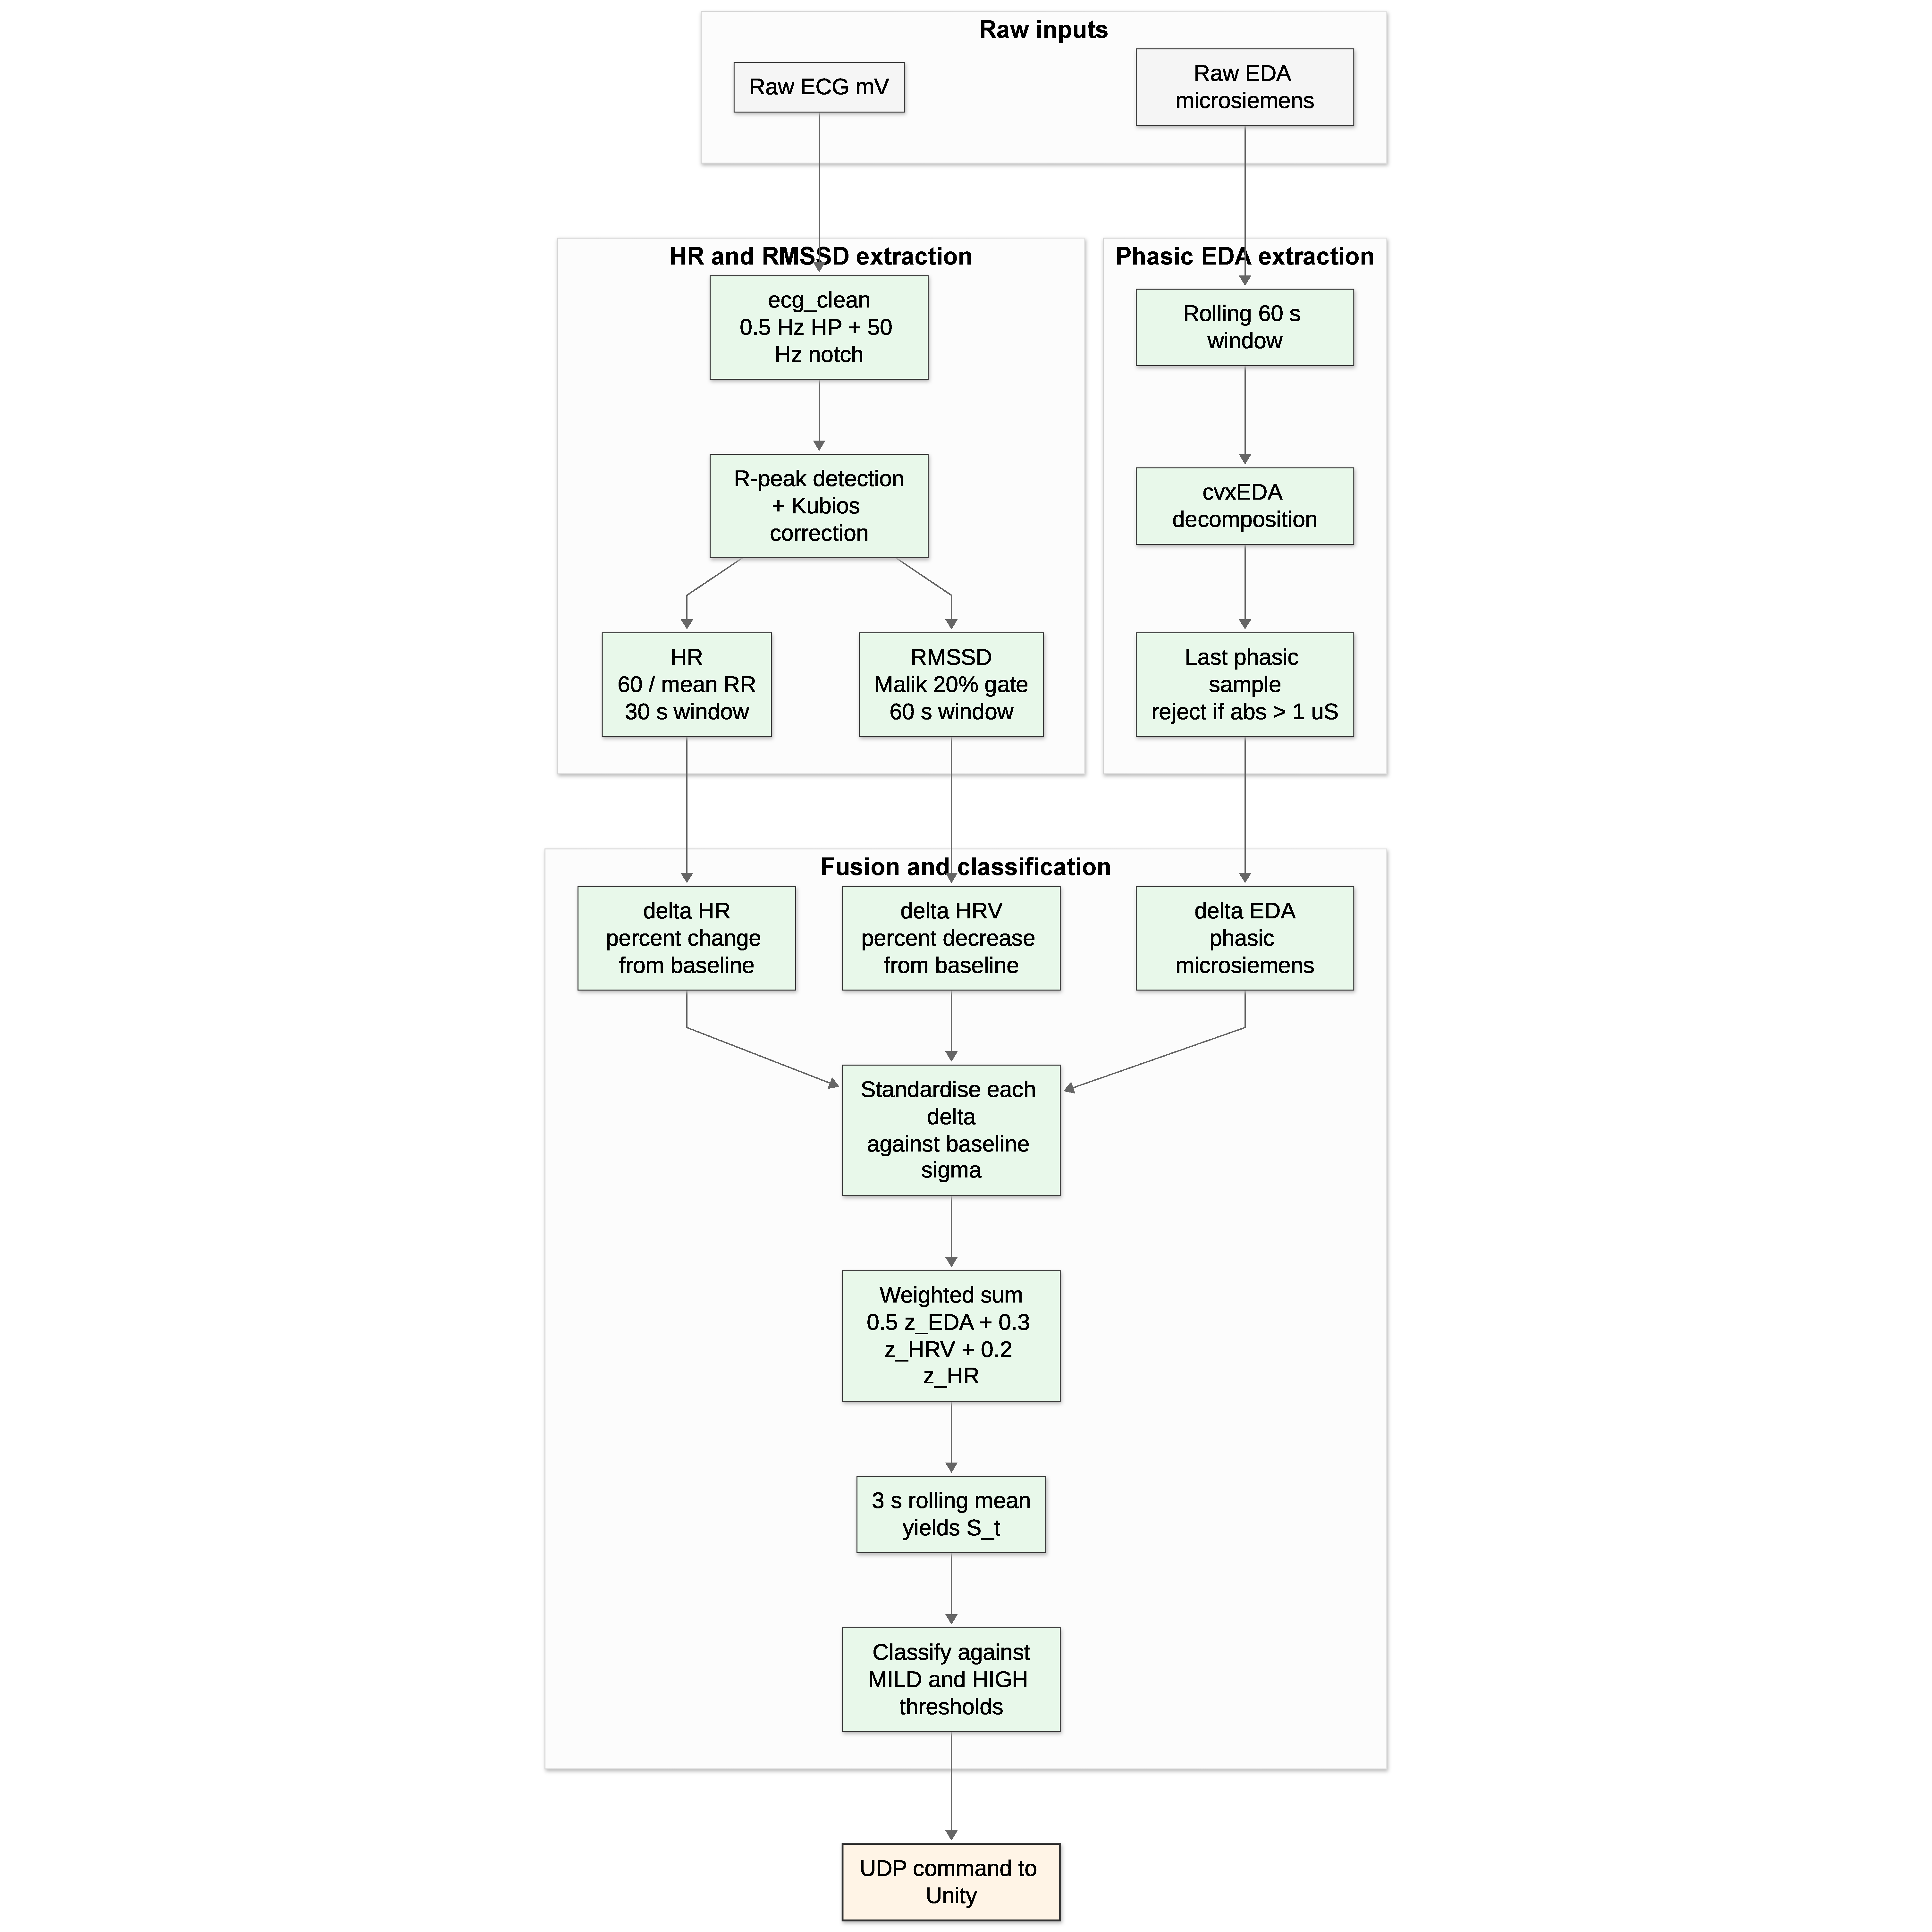
\includegraphics[width=\linewidth, height=0.9\textheight, keepaspectratio]{diagrams/03_signal_processing_chain.pdf}%
    }{%
        \fbox{\parbox{0.9\linewidth}{\centering
            \vspace{1.5cm}
            \textbf{[Diagram 3 placeholder, processing chain]}\\[6pt]
            \small Render the corresponding mermaid source and place
            the exported file in \texttt{diagrams/}.
            \vspace{1.5cm}
        }}%
    }
    \caption{Processing chain. The electrocardiogram yields heart
    rate and RMSSD; the conductance channel yields its phasic
    component; the three are standardised against the calibration
    reference, combined under fixed coefficients, and smoothed
    into the composite driving classification.}
    \label{fig:chain}
\end{figure}

% ,,,,,,,,,,,,,,,,,,,,,,
\subsection{Classification and closed-loop control}
\label{sec:control}
% ,,,,,,,,,,,,,,,,,,,,,,

\subsubsection{Threshold derivation}
\label{sec:thresholds}

Two thresholds partition the smoothed composite into three
states. Both are fixed at the close of calibration from the
dispersion of the unsmoothed composite over that same window:

\begin{align}
\theta_{\mathrm{MILD}} &= \mu_{S_{t}}^{\mathrm{cal}}
+ 1.28 \cdot \sigma_{S_{\mathrm{inst}}}^{\mathrm{cal}} \\[2pt]
\theta_{\mathrm{HIGH}} &= \mu_{S_{t}}^{\mathrm{cal}}
+ 2.33 \cdot \sigma_{S_{\mathrm{inst}}}^{\mathrm{cal}}
\end{align}

The coefficients 1.28 and 2.33 are the standard normal deviates
at the 90th and 99th percentiles. Were the unsmoothed composite
normally distributed at rest, it would exceed the two thresholds
about 10\% and 1\% of the time; the smoothed composite that is
actually classified varies less, so a participant at rest crosses
them less often still. Excursions above these bands during the
run therefore represent departures from that participant's own
resting distribution rather than arbitrary absolute levels, which
is what makes the bands transferable across participants without
retuning.

One asymmetry in the two expressions requires comment, since it
is easily read as an error. The dispersion is taken from the
unsmoothed series while the central value is taken from the
smoothed one. This is deliberate. A trailing mean reduces
dispersion, so a dispersion measured on the smoothed series would
be too small, narrowing the middle band and sending genuine
excursions from the lowest band directly to the highest. The central value may safely be taken
from the smoothed series because a mean is invariant under
trailing averaging.

For display, the composite is also mapped onto a score running
from 0 at the calibration mean through 50 at the lower threshold
to 100 at the upper one; the score plays no part in control.

\subsubsection{Control law}
\label{sec:controllaw}

The mapping from state to command is deterministic and admits no
intermediate cases:

\begin{itemize}
    \item $S_{t} \le \theta_{\mathrm{MILD}}$, the lowest band:
    the system emits \texttt{increase}. The environment responds
    by intensifying its stimulus, within whatever bounds that
    scenario defines.
    \item $\theta_{\mathrm{MILD}} < S_{t} \le \theta_{\mathrm{HIGH}}$,
    the middle band: no command is emitted and the environment
    holds its current configuration.
    \item $S_{t} > \theta_{\mathrm{HIGH}}$, the upper band: the
    system emits \texttt{decrease}. The environment reduces its
    stimulus.
\end{itemize}

Stated plainly, the loop drives the participant towards the
middle band and holds them there. Sustained low arousal produces
repeated \texttt{increase} commands and the stimulus escalates
until arousal enters the middle band, at which point escalation
ceases. Arousal above the upper threshold produces
\texttt{decrease} and the stimulus is withdrawn until arousal
returns. The middle band is thus not a target the system
approaches asymptotically but an interval within which it takes
no action at all.

How each scenario realises \texttt{increase} and
\texttt{decrease} is defined by that scenario and constitutes the
one respect in which the environments differ from one another.
The bounds within which escalation operates, the increment per
command, and the mapping from command to visible change are
properties of the environment rather than of the measurement
system, and are reported alongside the scenario descriptions.

\subsubsection{Command gating and rate limiting}
\label{sec:gating}

Two mechanisms sit between classification and transmission.

A \textbf{settling gate} withholds commands at the start of each
run, because the participant may still be adjusting the display
or settling into position and the earliest readings are
unrepresentative. For the first 3.5~s no command is sent whatever
the state; the interval exceeds the three seconds the smoothing
window takes to fill, so the provisional value the composite
reports meanwhile cannot open the gate. Thereafter the gate opens
at the first reading in the lowest band and remains open for the
rest of the run, while any other reading keeps it closed.

A \textbf{rate limit} permits at most one command per second.
Commands generated while the limit is in force are discarded
rather than queued, so the environment never receives a burst of
accumulated instructions after a quiet interval. This matters
because arousal oscillating near a threshold would otherwise
produce rapid alternation between escalation and withdrawal,
which is perceived as erratic. Discarding rather than queuing
also guarantees that every command the environment receives
reflects the current state rather than a state that has since
been superseded.

Every transmitted command is written to the session record with
its timestamp, the state and composite value producing it, and
the gate status at the time, which permits the exposure trajectory to be reconstructed
independently of the physiological traces.

\begin{figure}[H]
    \centering
    \IfFileExists{diagrams/05_feedback_loop_detail.png}{%
        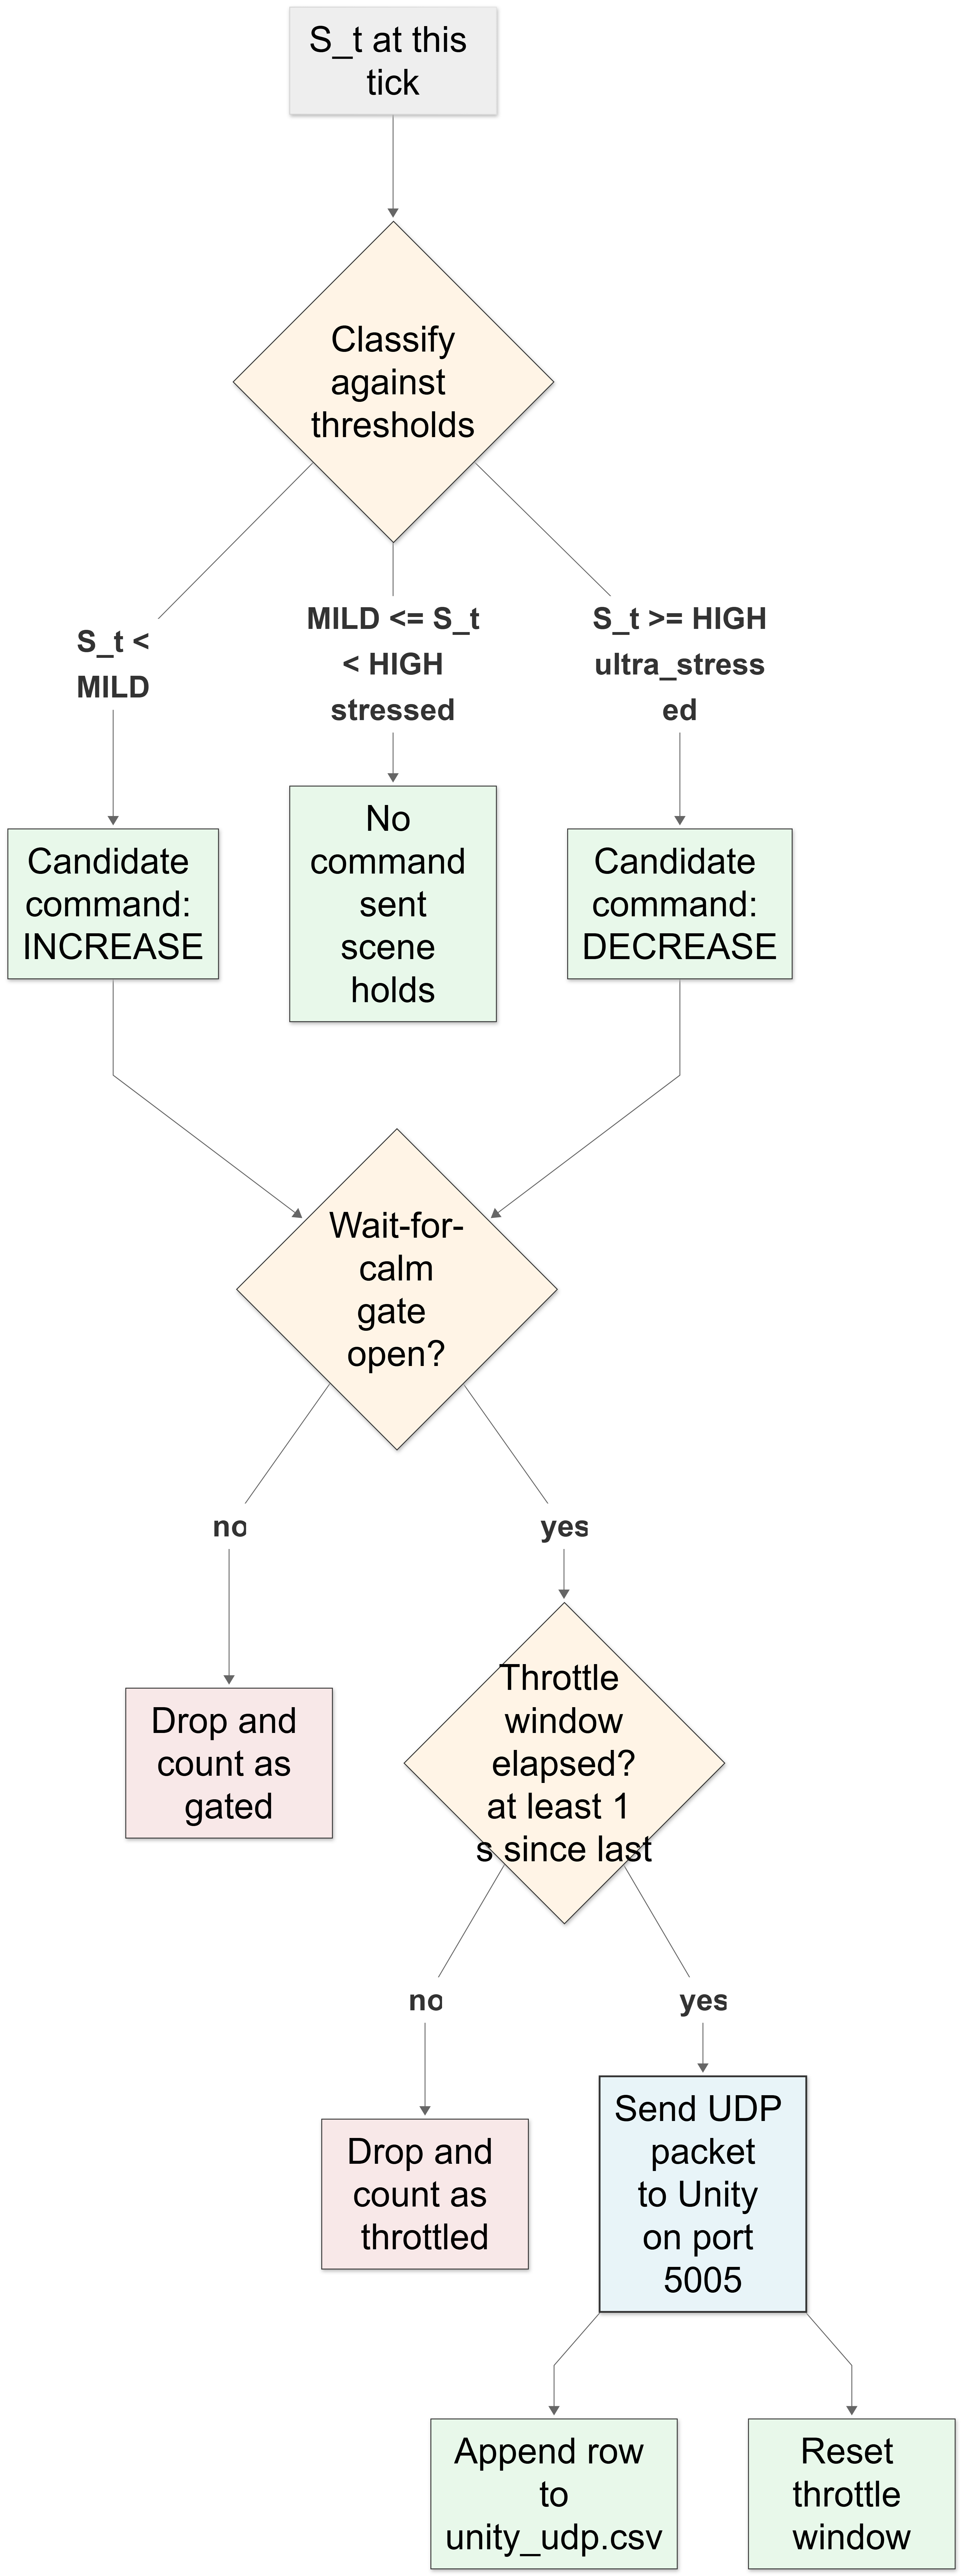
\includegraphics[width=\linewidth, height=0.9\textheight, keepaspectratio]{diagrams/05_feedback_loop_detail.png}%
    }{%
        \fbox{\parbox{0.9\linewidth}{\centering
            \vspace{1.5cm}
            \textbf{[Diagram 5 placeholder, control loop]}\\[6pt]
            \small Render the corresponding mermaid source and place
            the exported image in \texttt{diagrams/}.
            \vspace{1.5cm}
        }}%
    }
    \caption{The control loop at single-sample resolution. A
    classified state becomes a candidate command, which the
    settling gate and the rate limit filter before transmission.
    Every transmitted command is recorded.}
    \label{fig:loop}
\end{figure}

% ,,,,,,,,,,,,,,,,,,,,,,
\subsection{Virtual environment interface}
\label{sec:interface}
% ,,,,,,,,,,,,,,,,,,,,,,

The interface is deliberately asymmetric in the two directions.

\textbf{Outbound} commands are single UTF-8 strings, one per
UDP datagram to port 5005, drawn from a closed set of four. \texttt{start} and
\texttt{stop} delimit the run. \texttt{increase} and
\texttt{decrease} carry the control decision of
Section~\ref{sec:controllaw}. The measurement system attaches no
meaning to how any of these is realised.

\textbf{Inbound} telemetry arrives as UDP datagrams on port 5006
and uses one envelope for every scenario:

\begin{quote}\texttt{\{"scenario": "<name>", "data": \{<field>: <value>, \dots\}\}}\end{quote}

The envelope is treated as opaque. The scenario label identifies
the environment; the fields within are recorded verbatim. The
record declares no permissible fields, which is precisely what
allows a new scenario to be introduced without modifying the
measurement system; the console's display hints are optional, and
for a scenario without one it charts the first numeric field it
receives.

% ,,,,,,,,,,,,,,,,,,,,,,
\subsection{Scenario implementations}
\label{sec:unity-placeholder}
% ,,,,,,,,,,,,,,,,,,,,,,

\noindent
\fbox{\parbox{0.97\linewidth}{%
    \textbf{To be completed.}\\[4pt]
    \small
    This subsection reports the environments themselves: the
    stimulus each presents, the bounds within which escalation
    operates, the increment applied per command, and the mapping
    from command to visible change. Reviewers of related work
    have asked specifically for numerical bounds here, so each
    scenario should state its range explicitly rather than
    describing escalation qualitatively.
}}

\vspace{6pt}
\noindent
Each scenario description should report:

\begin{itemize}
    \item the stimulus presented and its physical or spatial
    range, stated numerically;
    \item the increment applied on each \texttt{increase} and
    \texttt{decrease}, and any limit on cumulative change;
    \item environment design, including visual and auditory
    composition, with reference to the presence literature where
    design decisions rest on it
    \citep{slater2009, diemer2015, bailenson2003};
    \item participant interaction available within the
    environment, and any input device used;
    \item measures taken against simulator discomfort, and the
    means by which a participant terminates the session
    themselves;
    \item the telemetry fields the environment emits and their
    units.
\end{itemize}

% ,,,,,,,,,,,,,,,,,,,,,,
\subsection{Session procedure}
\label{sec:procedure}
% ,,,,,,,,,,,,,,,,,,,,,,

Each session proceeds through five phases. Apart from the close of
the calibration window, which the system performs itself once
120~s have elapsed, every transition is initiated by the operator,
and the state of the system determines which controls are
available at any moment.

\begin{enumerate}
    \item \textbf{Preparation.} The participant is briefed on the
    procedure and on the means of terminating the session.
    Written consent is obtained. Electrode sites are cleaned and
    sensors applied as described in Section~\ref{sec:sensing}.
    Signal quality is verified on the console before proceeding.
    \item \textbf{Settling.} The participant sits quietly while
    the calibration control remains locked, for the interval
    described in Section~\ref{sec:interlock}. Conductance in
    particular requires several minutes for electrode hydration
    to stabilise, and a calibration taken before it has done so
    yields a drifting reference.
    \item \textbf{Calibration.} The 120~s window of
    Section~\ref{sec:calibration} runs with the environment
    inactive. On completion the reference values, dispersions and
    thresholds are fixed, checked for validity as described in
    Section~\ref{sec:validity}, and written to the session record.
    \item \textbf{Run.} The environment starts and the control
    loop of Section~\ref{sec:control} operates. Duration is
    determined by the protocol rather than by the measurement
    system, which imposes no limit of its own.
    \item \textbf{Termination.} The operator stops the run, or
    the participant terminates it, or a monitoring condition from
    Section~\ref{sec:safety} triggers. Records are closed and
    written.
\end{enumerate}

\begin{figure}[H]
    \centering
    \IfFileExists{diagrams/04_session_state_machine.png}{%
        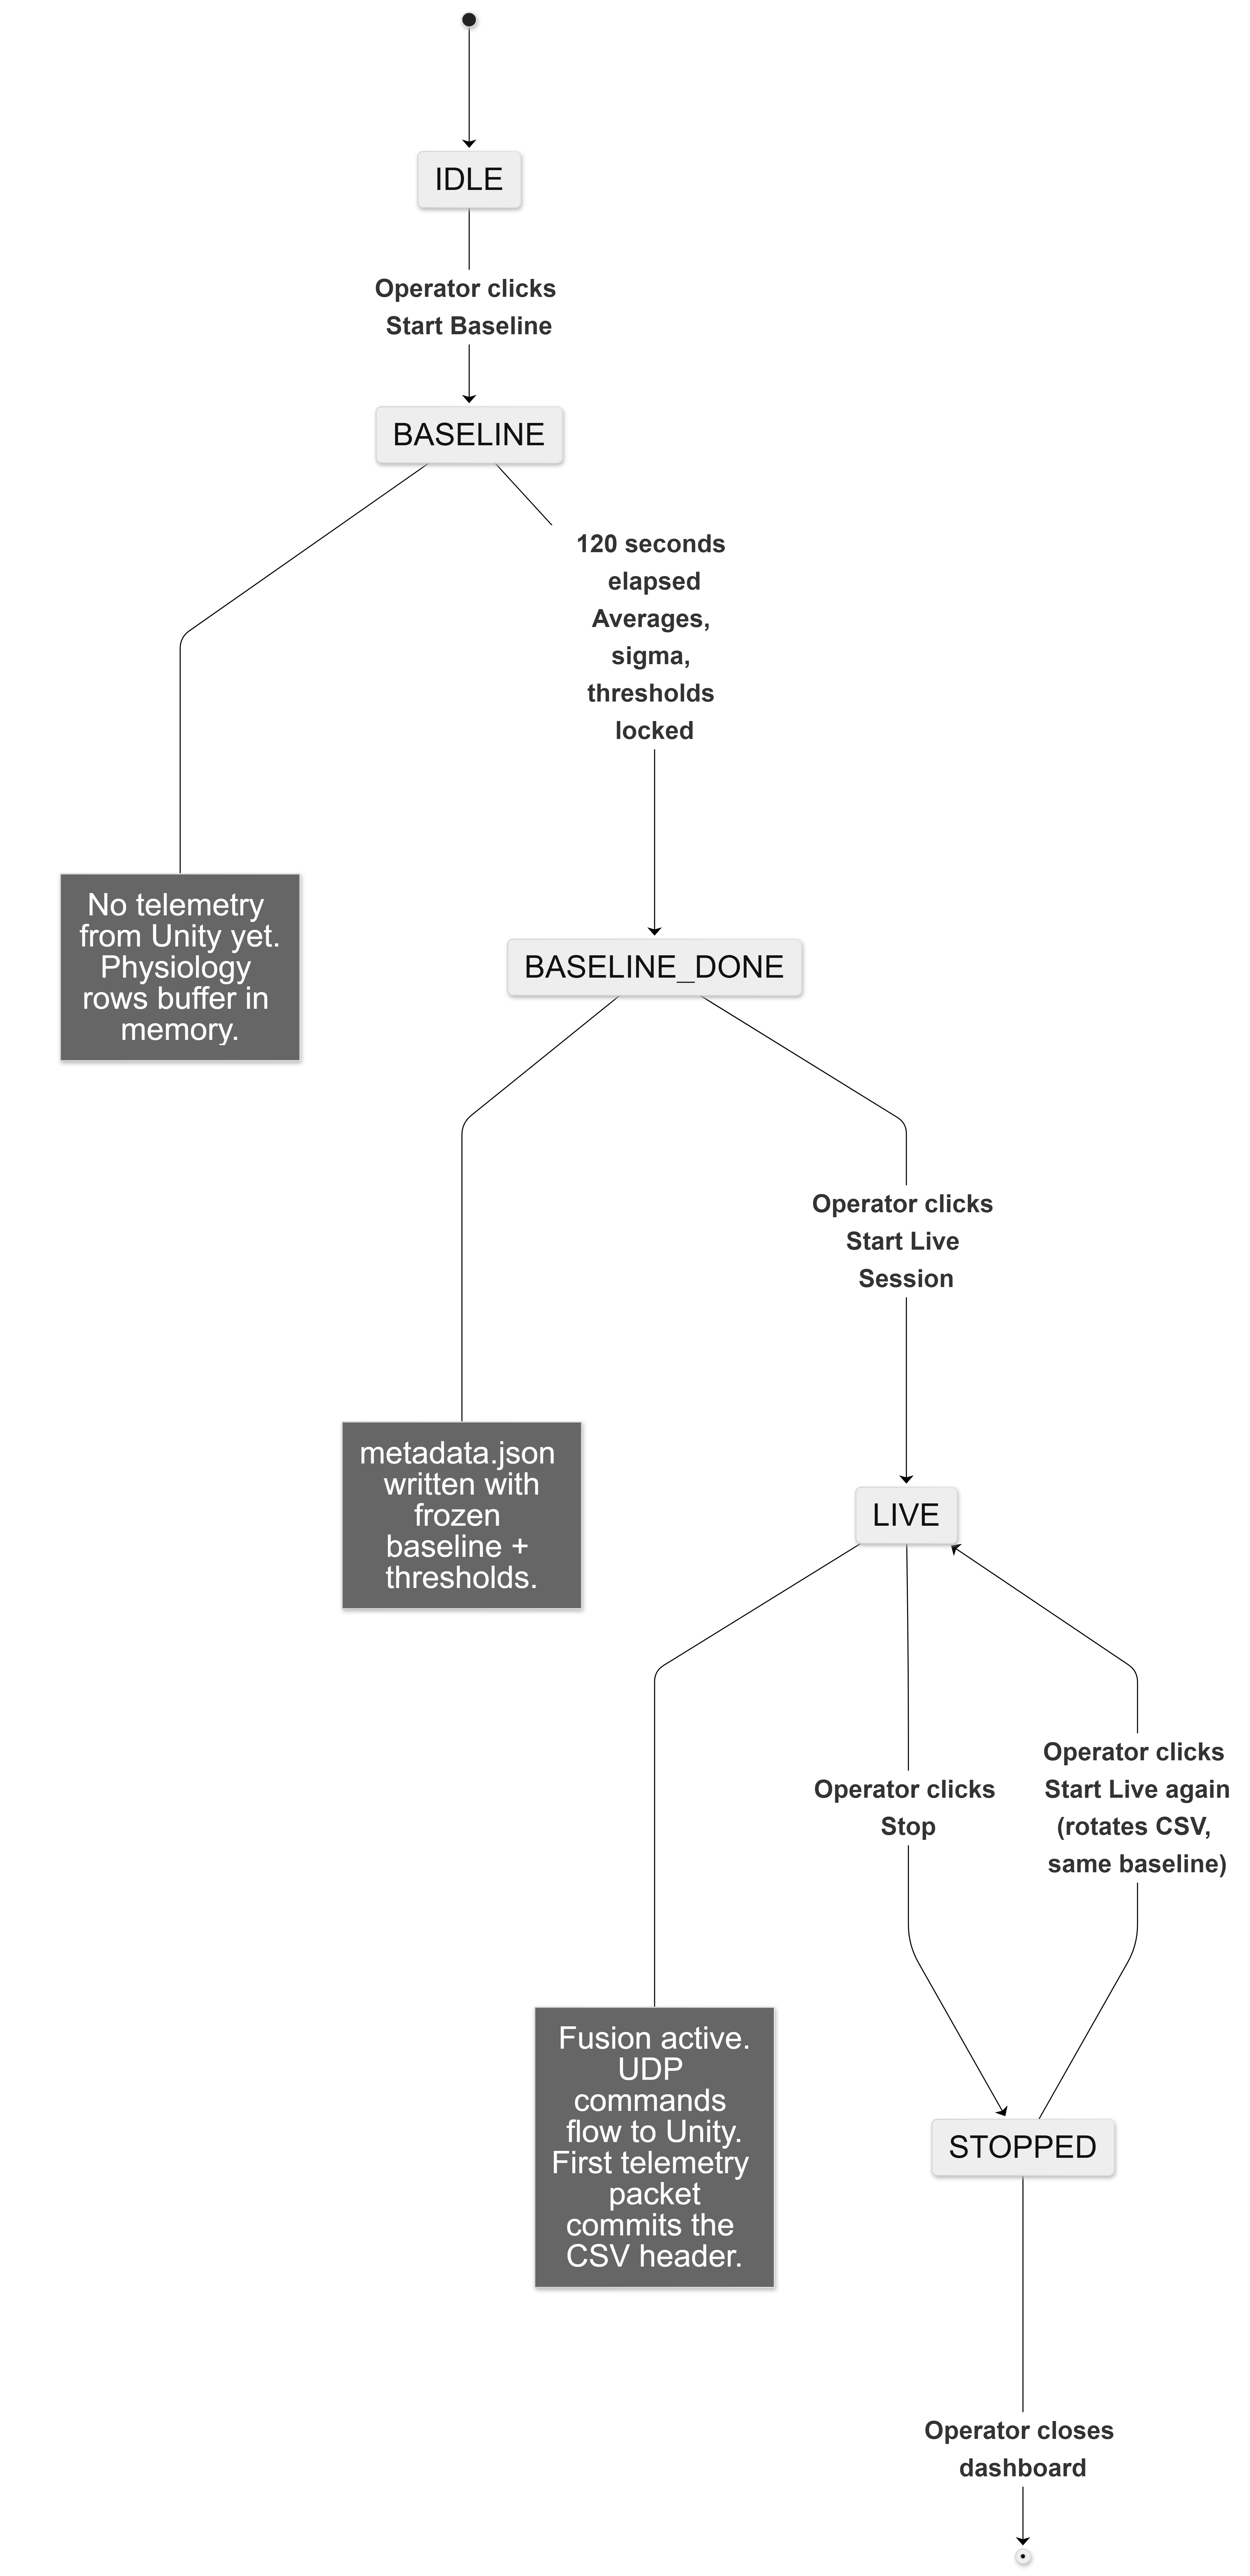
\includegraphics[width=\linewidth, height=0.9\textheight, keepaspectratio]{diagrams/04_session_state_machine.png}%
    }{%
        \fbox{\parbox{0.9\linewidth}{\centering
            \vspace{1.5cm}
            \textbf{[Diagram 4 placeholder, session states]}\\[6pt]
            \small Render the corresponding mermaid source and place
            the exported image in \texttt{diagrams/}.
            \vspace{1.5cm}
        }}%
    }
    \caption{Session state progression. The operator advances the
    system through each phase explicitly, except that calibration
    closes by itself when its window has elapsed. Completion of
    calibration fixes the thresholds, and entry to the run opens
    the command channel.}
    \label{fig:state}
\end{figure}

At least two people are present throughout: an operator
responsible for the console and for observing the participant,
and a second person responsible for the environment and for
assisting with the display. Neither leaves the room while a
participant is wearing the display.

Each launch of the system serves exactly one participant, and a
new participant begins with a new launch; the reasons, and the
handling of repeated attempts within a launch, are set out in
Section~\ref{sec:integrity}.

\subsubsection{Calibration interlock}
\label{sec:interlock}

The calibration control is locked for a configurable interval
after launch and unlocks once that interval has elapsed, with the
remaining time displayed on the control itself so the delay reads
as intentional rather than as a fault.

Two considerations motivate the lock. RMSSD is estimated over a
60~s trailing window, so an operator beginning calibration
immediately would spend the first half of a 120~s window
accumulating no variability data at all, and the resulting
dispersion would rest on half the intended sample. Separately,
electrode hydration requires time to stabilise, and a reference
taken during that transient is not the resting value it is
supposed to represent.

The default is 60~s, aligning the lock with the variability
window. A protocol adopting the 300~s figure
of~\citet{taskforce1996} raises the constant accordingly, with no
other modification required. Nothing in the composite arithmetic
or the threshold derivation is affected by the choice.

\subsubsection{Operator console}
\label{sec:console}

All operator interaction passes through a console on the
workstation. It holds no processing logic: each control publishes
a message on an internal stream that the main process consumes,
and the main process broadcasts its state back on a second
stream, from which the console determines which controls to
enable. Neither imports from the other.

A dialogue precedes the pipeline and captures what is required to
name the session directory and satisfy the arrangements of
Section~\ref{sec:ethics}. Three fields are entered: a
laboratory-assigned participant code of up to thirty-two letters,
digits, hyphens or underscores, which names the directory and is
not resolvable to an individual outside the laboratory's separate
register; sex, recorded as a closed selection with neither option
preselected, since free text accumulates inconsistent entries
requiring reconciliation before any aggregate analysis, and a
preselected default would be recorded silently whenever the field
was overlooked; and
session number, bounded above by a configuration constant
presently set to three. The session date is added automatically.
Given name and family name were recorded
by earlier revisions and are no longer written to any file the
system produces.

The console window divides into a calibration panel and a run
panel. The calibration panel counts down the window and displays
a running mean of the three measures refreshed every ten seconds,
so the operator observes the estimates settling rather than
waiting against an empty display; on completion it presents the
fixed reference values, the dispersion of the composite, both
thresholds and the number of samples excluded as artifact. The run
panel
remains inert until calibration completes, and stays inert if
the calibration fails the check of Section~\ref{sec:validity}, in
which case the reason is displayed in its place. A run may be
repeated without repeating the calibration: after confirmation the
previous run is replaced while the calibration is retained, so an
interruption does not cost the calibration window. Current state
is displayed as a single indicator and the smoothed composite is
plotted alongside its three constituents. A further panel charts
one telemetry field, the one named by the display hint for a known
scenario or otherwise the first numeric field received, and reports
plainly when no environment is connected. A trace of the last six
seconds of electrocardiogram lets the operator judge electrode
contact, a red banner announces loss of signal once the sensor has
been silent for about two and a half seconds, and stopping a run
asks the operator whether to finish and save or to stay.

% ,,,,,,,,,,,,,,,,,,,,,,
\subsection{Monitoring and session termination}
\label{sec:safety}
% ,,,,,,,,,,,,,,,,,,,,,,

Three independent mechanisms can end a session, and they are
described together because the system is designed so that no one
of them is relied upon alone.

\textbf{Participant termination.} The participant is informed
before the session begins that they may stop at any point, for
any reason, without explanation, and that doing so carries no
consequence for their participation. The means of stopping is
demonstrated rather than merely described. This takes precedence
over every other consideration and requires no operator
concurrence.

\textbf{Operator termination.} The operator observes both the
participant and the console throughout. Termination follows
visible distress, a request for a pause, or any physical sign
inconsistent with the traces on screen. The operator is not
required to justify stopping and is instructed to resolve
uncertainty in favour of stopping.

\textbf{Automatic safeguards.} The validity bounds of
Section~\ref{sec:acquisition} serve a monitoring function
alongside their signal-processing one. A heart rate above 220 or
below 30 beats per minute is not treated as a measurement: the last
valid value is held in its place, since such a reading indicates
either sensor failure or a state that the operator rather than the
control loop should judge. A sensor that falls silent is handled as
described below, and a silence lasting fifty seconds ends the
session, with everything recorded up to that point kept and the
environment told to stop.

The control law itself provides a fourth, softer mechanism. Because
arousal above the upper threshold produces \texttt{decrease}
rather than escalation, the loop withdraws stimulus as arousal
rises. A participant whose arousal continues climbing therefore
encounters a diminishing rather than an intensifying environment,
and the design contains no path by which sustained high arousal
produces further escalation.

Three properties of the arrangement are worth stating explicitly.
The measurement system never acts in the absence of a recent
valid measurement. A silence from the sensor unit longer than half
a second, as when its wireless link drops, is no longer bridged,
so the samples it last delivered stop being passed on as though
they were current; once no fresh sample has arrived for two
seconds no further command is sent, and the environment holds
where it stands until samples resume. A silence persisting beyond
fifty seconds ends the session. A channel that stays connected but
stops varying, the signature of a detached electrode or of a
saturated sensor, raises a warning rather than halting the loop,
since the remaining channels still carry information and a
saturated conductance channel may reflect genuine sweating.
The settling gate holds every command until the composite,
computed over a full smoothing window, first reads in the lowest
band.
Finally, no run can begin on a calibration that failed the check
of Section~\ref{sec:validity}: the run control is withheld on the
console, and the pipeline refuses the command on its own account.

% ,,,,,,,,,,,,,,,,,,,,,,
\subsection{Data recording}
\label{sec:recording}
% ,,,,,,,,,,,,,,,,,,,,,,

Each session produces one directory containing four files, to
which a spreadsheet copy of the session record is added whenever a
run stops.

\textbf{The session record} holds, at the 10~Hz processing rate
and during calibration and runs only, the participant code and
session details, the phase, the physiological values as delivered
to the pipeline, the three deviations, the composite before and
after smoothing, the state with its display score, whatever
telemetry the environment is emitting, and the number of
calibration samples excluded as artifact. Each row is written to
disk at the
moment it is recorded. Calibration ordinarily precedes any
telemetry from the environment, so the earliest rows are written
under a header carrying physiological columns alone; when the
first non-empty telemetry packet arrives, the header gains the
fields it names and each row already on disk gains matching empty
cells, so that every row continues to align with its header. No
row is ever held in memory awaiting a schema, and an interruption
at any point loses nothing already recorded.

\textbf{The diagnostic trace} records the raw value of every
channel at every internal processing step, together with an
acquisition status code distinguishing a fresh sample from a held
one, an out-of-bounds rejection, and an invalid reading. This
permits reconstruction of exactly what the system observed at any
instant. The file is verbose but small, a few hundred kilobytes
for a typical session.

\textbf{Session metadata} is written as structured text and
contains the pre-session record, the fixed reference values, the
dispersion of the calibration composite, both thresholds, the
number of samples excluded, the data source and the processing
constants in force, the verdict on whether the calibration is
usable together with its reasons
(Section~\ref{sec:validity}), and the scenario label learned from
the first telemetry packet. It is written once at session start
and amended at the close of calibration.

\textbf{The command log} records every transmitted command with
timestamp, originating state, composite value and gate status,
as described in
Section~\ref{sec:gating}.

\subsubsection{Repeated attempts and record integrity}
\label{sec:integrity}

One launch of the system serves one participant, by design. The
session directory is bound at launch to a single participant code,
and the calibration established within it describes that
participant's resting physiology and nobody else's. Admitting a
second participant into a running launch would score them against
another person's reference values, silently and with no trace in
the record. The procedure is therefore built around a single
sequence of calibration, exposure and recording, and a new
participant begins with a new launch.

Within a launch either phase may be repeated, and a repetition
replaces what it supersedes rather than accumulating beside it.
Repeating the calibration discards everything recorded so far in
that launch, the run included, because a run is interpretable only
against the calibration that preceded it. Repeating the run
discards the previous run while retaining the calibration and the
rows recorded during it, so the resting trace that produced the
reference values survives any number of repeated runs. Abandoning
a calibration before its window completes discards it, since an
incomplete window cannot yield thresholds. Stopping a run, by
contrast, discards nothing.

Every action that would discard recorded data asks first, names
what will be lost, and offers cancellation as the default
response, so that neither an inadvertent keystroke nor a double
click can destroy a recording. At the close of a launch the
operator chooses to keep everything, to keep the calibration
alone, or to discard both. A launch interrupted from the terminal
rather than closed through that dialogue keeps everything it
recorded, on the principle that a record can always be deleted
afterwards but cannot be recovered once discarded.

These properties are made observable rather than merely asserted.
The console reports continuously how many calibration rows and how
many run rows are on disk, so that an operator can confirm, while
the participant is still present, that a repetition replaced its
rows instead of appending to them.

% ,,,,,,,,,,,,,,,,,,,,,,
\subsection{Validation and reproducibility}
\label{sec:reproducibility}
% ,,,,,,,,,,,,,,,,,,,,,,

Two provisions make what the system reports checkable: an
independent implementation against which its derived quantities
can be compared, and properties that let any run be repeated on
identical input.

\subsubsection{Cross-validation of the extraction backends}
\label{sec:crossval}

Agreement is quantified by driving both backends over one
archived recording and comparing their outputs sample by sample.
Because the input is identical, no alignment or resampling step
is required and every difference is attributable to extraction.

Three quantities are compared: heart rate, RMSSD, and the
composite index that both feed. For each, we report Pearson
correlation over samples where both backends return a valid
value, root mean square difference, and mean signed difference to
expose systematic offset as distinct from scatter. RMSSD is
additionally compared over clean segments alone, since the two
implementations apply different criteria for excluding intervals
and the comparison over all samples conflates disagreement about
values with disagreement about which samples are admissible.

An accompanying script performs this comparison over any raw
capture file and emits both the figures and the underlying values.
The agreement obtained is reported in
Section~\ref{sec:results-backends}, and extending the comparison
across the full recorded set requires no further implementation.

\subsubsection{Properties supporting reproduction}

Five properties of the implementation support reproduction.

\textbf{Deterministic replay.} The replay source waits for its
consumer to subscribe before emitting, so identical input yields
identical output. This was not originally the case, and
the defect it corrected is described in
Section~\ref{sec:data-source}.

\textbf{Fixed conversion constants.} Conversion from converter
integers, applied only to archived recordings since live capture
supplies physical units, uses constants fixed in one location and
documented per channel.

\textbf{Independent extraction.} Any claim resting on derived
quantities can be checked against a second implementation, as
described in Sections~\ref{sec:backends} and~\ref{sec:crossval}.

\textbf{Complete diagnostic trace.} The raw value and acquisition
status at every processing step are recorded, so any anomaly in
the session record can be traced to what the system observed.

\textbf{Complete command log.} Every transmitted command is
recorded, so the exposure trajectory is reconstructible
independently of the physiological traces.

% ,,,,,,,,,,,,,,,,,,,,,,
\subsection{Ethics and data protection}
\label{sec:ethics}
% ,,,,,,,,,,,,,,,,,,,,,,

The arrangements below reflect decisions taken by the supervising
investigator and the laboratory administration and apply from the
present version of the system. Recordings collected before the
identifier reduction described here remain on file under the
earlier schema and will be pseudonymised before any transfer
outside the laboratory.

Written informed consent is obtained before every session.
Consent covers recording of the two physiological channels,
storage of the derived quantities, and the right to withdraw at
any point. Withdrawal results in deletion of that participant's
records; because no cross-reference to the participant exists
outside the session directory, deletion is a single operation on
a single directory.

Identifiers written to disk are limited to the laboratory-assigned
participant code, sex, session number and session date. Neither
given name nor family name is written to any file the system
produces. Session directories are named by participant code,
session number, date and sex.

The laboratory administrator at the NISC laboratory, University
of Messina, acts as data controller, and requests for access,
correction or erasure are directed there.

Recordings are retained for five years and derived research
outputs for ten, after which each is destroyed. Storage is on the
laboratory workstation, access to which is physically controlled.
Encryption at rest is not presently implemented. Data is
transferred only on explicit request and by direct transfer; no
cloud service, backup provider or code repository holds a copy.

\textit{Ethical approval reference to be inserted before
submission.}
